\documentclass{ctexart}
\usepackage{PhysicalChemistryNote}

\begin{document}\pagestyle{plain}
\Section{7D.1 链反应动力学}
\Part{链反应的基本概念}
\indent 在化学动力学中有一类特殊的反应,只需用热,光或辐射等方法使反应引发,%
体系就能通过活性组分(通常是自由基或原子)相继发生一系列的连续反应,%
像链条一样自动地发展下去.
\begin{definition}[7D.1.1 链反应]
    \tbf{链反应}(又称\tbf{连锁反应}),是指反应的产物或副产物又可作为其他反应的原料,%
    从而使反应反复发生.在化学中,链反应通常在光,热,辐射或引发剂作用下,反应中交替产生活性中间体(如自由原子或自由基),%
    从而使反应一直进行下去.
\end{definition}
按照活性物质数量的变化,链反应主要有三个过程.
\begin{definition}[7D.1.2 链反应的过程]
    在链反应中,产生活性中间体的过程称为\tbf{链引发},%
    活性中间体与反应物分子反复作用生成产物的过程称为\tbf{链增长}或\tbf{链传递},%
    活性中间体最后湮灭的过程称为\tbf{链终止}.
\end{definition}
一般的链增长过程中,一个活性中间体产生一个新的活性中间体.例如\ce{Cl.}与\ce{H2}的反应:
\begin{tightcenter}
    \ce{Cl. + H2 -> HCl + H.}
\end{tightcenter}
不过,在部分链增长过程中,一个活性中间体也可能产生数个活性中间体.例如\ce{H.}与\ce{O2}的反应:
\begin{tightcenter}
    \ce{H. + O2 -> HO. + O.}
\end{tightcenter}
据此,我们可以按照链增长的性质对链反应进行分类.
\begin{definition}[7D.1.3 直链反应与支链反应]
    一个活性中间体只能产生一个新的活性中间体的反应称为\tbf{直链反应},%
    可以产生两个或多个新的活性中间体的反应称为\tbf{支链反应}.
\end{definition}
我们将在接下来对这些链反应的速率方程进行详细地讨论.\vspace{4pt}\\
\Part{简单直链反应——\ce{H2}与卤素单质的自由基反应}
\indent 对中间体与总反应速率的研究表明,\ce{H2}与\ce{X2}(其中$\ce{X}=\ce{Cl},\ce{Br}$)在光照或加热下的化合反应%
的机理是不同的.我们先从最简单的\ce{H2}与\ce{Cl2}的反应开始.\ce{H2}与\ce{Cl2}通过自由基反应生成\ce{HCl}的反应机理如下.
\begin{tightcenter}
    \ce{Cl2 <=>T[$k_1$][$k_{-1}$] 2Cl.}\\
    \ce{Cl. + H2 ->T[$k_2$] HCl + H.}\\
    \ce{H. + Cl2 ->T[$k_3$] HCl + Cl.}
\end{tightcenter}
由于产物\ce{HCl}十分稳定,因此忽略后两个反应的逆反应.现在我们来推导该体系的反应速率方程.
\begin{derivation}\setcounter{equation}{0}
    体系中的不稳定中间体为\ce{H.}与\ce{Cl.},分别对它们稳态近似有
    \begin{equation}
        \dfrac{\di\con{H.}}{\di t}=k_2\con{Cl.}\con{H2}-k_3\con{H.}\con{Cl2}=0
    \end{equation}
    \begin{equation}
        \dfrac{\di\con{Cl.}}{\di t}=2k_1\con{Cl2}-2k_{-1}\con{Cl.}^2-k_2\con{Cl.}\con{H2}+k_3\con{H.}\con{Cl2}=0
    \end{equation}
    将(2)减去(1)可得
    \begin{equation}
        2k_1\con{Cl2}-2k_{-1}\con{Cl.}^2=0
    \end{equation}
    于是
    \begin{equation}
        \con{Cl.}=\sqrt{\dfrac{k_1}{k_{-1}}\con{Cl2}}
    \end{equation}
    由(1)可得
    \begin{equation}
        \dfrac{\di\con{HCl}}{\di t}=k_2\con{Cl.}\con{H2}+k_3\con{H.}\con{Cl2}=2k_2\con{Cl.}\con{H2}
    \end{equation}
    将(4)代入(5)可得
    \begin{equation}
        \dfrac{\di\con{HCl}}{\di t}=2k_2\con{Cl.}\con{H2}=2k_2\sqrt{\dfrac{k_1}{k_{-1}}}\con{H2}\con{Cl2}^{\frac12}
    \end{equation}
    因此反应对\ce{H2}为一级,对\ce{Cl2}为二分之一级.
\end{derivation}
而\ce{H2}与\ce{Br2}的反应就略微复杂一些.两者通过自由基反应生成\ce{HBr}的反应机理如下.
\begin{tightcenter}
    \ce{Br2 <=>T[$k_1$][$k_{-1}$] 2Br.}\\
    \ce{Br. + H2 <=>T[$k_2$][$k_{-2}$] HBr + H.}\\
    \ce{H. + Br2 ->T[$k_3$] HBr + Br.}
\end{tightcenter}
由于\ce{HBr}相对不那么稳定,并且\ce{H.}的能量很高,因此相比\ce{HCl}需要额外考虑%
\ce{HBr}与\ce{H.}的反应.
\begin{derivation}\setcounter{equation}{0}
    体系中的不稳定中间体为\ce{H.}与\ce{Br.},分别对它们稳态近似有
    \begin{equation}
        \dfrac{\di\con{H.}}{\di t}=k_2\con{Br.}\con{H2}-k_{-2}\con{H.}\con{HBr}-k_3\con{H.}\con{Br2}=0
    \end{equation}
    \begin{equation}
        \dfrac{\di\con{Br.}}{\di t}=2k_1\con{Br2}-2k_{-1}\con{Br.}^2-k_2\con{Br.}\con{H2}+k_{-2}\con{H.}\con{HBr}+k_3\con{H.}\con{Br2}=0
    \end{equation}
    将(2)减去(1)可得
    \begin{equation}
        2k_1\con{Br2}-2k_{-1}\con{Br.}^2=0
    \end{equation}
    于是
    \begin{equation}
        \con{Br.}=\sqrt{\dfrac{k_1}{k_{-1}}\con{Br2}}
    \end{equation}
    将(4)代入(1)可得
    \begin{equation}
        \con{H.}=\dfrac{k_2\con{Br.}\con{H2}}{k_{-2}\con{HBr}+k_3\con{Br2}}=\dfrac{k_2\sqrt{\dfrac{k_1}{k_{-1}}}\con{H2}\con{Br2}^{\frac12}}{k_{-2}\con{HBr}+k_3\con{Br2}}
    \end{equation}
    将(4)(5)代入$\dfrac{\di\con{HBr}}{\di t}$可得
    \begin{equation}
        \dfrac{\di\con{HBr}}{\di t}=k_2\con{Br.}\con{H2}+k_3\con{H.}\con{Br2}-k_{-2}\con{HBr}\con{H.}=\dfrac{2k_2k_3\sqrt{\dfrac{k_1}{k_{-1}}}\con{H2}\con{Br2}^{\frac32}}{k_3\con{Br2}+k_{-2}\con{HBr}}
    \end{equation}
    令$k_a=2k_3\sqrt{\dfrac{k_1}{k_{-1}}},k_b=\dfrac{k_{-2}}{k_2}$,就有
    \begin{equation}
        \dfrac{\di\con{HBr}}{\di t}=\dfrac{k_a\con{H2}\con{Br2}^{\frac32}}{\con{Br2}+k_b\con{HBr}}
    \end{equation}
    这就是我们在\tbf{7A.2}中给出的速率方程.
\end{derivation}
而\ce{H2}与\ce{F2}或\ce{I2}的反应则比较复杂,我们在这里就不叙述了.如果你感兴趣,可以自行查阅相关资料.\vspace{4pt}\\
\Part{复杂直链反应——自由基氧化}
\indent 脂类物质的氧化是油脂保存过程中广泛存在的问题.如果反应物记作\ce{RH},那么总反应方程式如下.
\begin{tightcenter}
    \ce{RH + O2 -> ROOH}
\end{tightcenter}
产生的过氧化物\ce{ROOH}可以进一步催化体系中其余\ce{RH}被\ce{O2}氧化.%
反应的机理如下.
\begin{tightcenter}
    \ce{2ROOH ->T[$k_1$] 2R. + \text{副产物}}\\
    \ce{R. + O2 ->T[$k_2$] ROO.}\\
    \ce{ROO. + RH ->T[$k_3$] ROOH + R.}\\
    \ce{2R. ->T[$k_4$] R2}\\
    \ce{R. + ROO. ->T[$k_5$] ROOR}\\
    \ce{2ROO. ->T[$k_6$] ROOR + O2}
\end{tightcenter}
实验表明有近似关系$4k_4k_6=k_5^2$.%
现在我们来考察这一自催化体系的速率方程(以\ce{O2}的消耗速率计).如果同时考虑三种链终止的方式,%
那么这对我们来说有些复杂,因此我们先从简单的情形入手.\\
\indent \tbf{Case I.} \ce{O2}浓度较低.
\begin{derivation}\setcounter{equation}{0}
    这时,体系中主要存在的自由基为\ce{R.},链终止步骤主要为\ce{2R. -> R2}.对体系中的两种自由基\ce{R.}和\ce{ROO.}做稳态近似可得
    \begin{equation}
        \dfrac{\di\con{R.}}{\di t}=2k_1\con{ROOH}^2-k_2\con{R.}\con{O2}+k_3\con{ROO.}\con{RH}-2k_4\con{R.}^2=0
    \end{equation}
    \begin{equation}
        \dfrac{\di\con{ROO.}}{\di t}=k_2\con{R.}\con{O2}-k_3\con{ROO.}\con{RH}=0
    \end{equation}
    $(1)-(2)$可得
    \begin{equation}
        2k_1\con{ROOH}^2-2k_4\con{R.}^2=0
    \end{equation}
    于是
    \begin{equation}
        \con{R.}=\sqrt{\dfrac{k_1}{k_4}}\con{ROOH}
    \end{equation}
    于是
    \begin{equation}
        -\dfrac{\di\con{O2}}{\di t}=k_2\con{R.}\con{O2}=k_2\sqrt{\dfrac{k_1}{k_4}}\con{ROOH}\con{O2}
    \end{equation}
    此时,反应对\ce{ROOH}和\ce{O2}均为一级.可以看到,%
    反应的速率随着产物\ce{ROOH}的增加而增加,因此随着反应进行,速率会逐渐加快.
\end{derivation}
\tbf{Case II.} \ce{O2}浓度较高.
\begin{derivation}\setcounter{equation}{0}
    这时,体系中主要存在的自由基为\ce{ROO.},链终止步骤主要为\ce{2ROO. -> ROOR + O2}.对体系中的两种自由基\ce{R.}和\ce{ROO.}做稳态近似可得
    \begin{equation}
        \dfrac{\di\con{R.}}{\di t}=2k_1\con{ROOH}^2-k_2\con{R.}\con{O2}+k_3\con{ROO.}\con{RH}=0
    \end{equation}
    \begin{equation}
        \dfrac{\di\con{ROO.}}{\di t}=k_2\con{R.}\con{O2}-k_3\con{ROO.}\con{RH}-2k_6\con{ROO.}^2=0
    \end{equation}
    $(1)+(2)$可得
    \begin{equation}
        2k_1\con{ROOH}^2-2k_6\con{ROO.}^2=0
    \end{equation}
    于是
    \begin{equation}
        \con{ROO.}=\sqrt{\dfrac{k_1}{k_6}}\con{ROOH}
    \end{equation}
    由(2)亦可得
    \begin{equation}
        -\dfrac{\di\con{O2}}{\di t}=k_2\con{R.}\con{O2}-k_6\con{ROO.}^2=k_3\con{ROO.}\con{RH}+k_6\con{ROO.}^2
    \end{equation}
    由于自由基\ce{ROO.}的浓度很低,链终止的速率远小于链增长的速率,因此可以近似地忽略后一项.于是有
    \begin{equation}
        -\dfrac{\di\con{O2}}{\di t}=k_3\sqrt{\dfrac{k_1}{k_6}}\con{ROOH}\con{RH}
    \end{equation}
    此时,反应对\ce{ROOH}和\ce{RH}均为一级.可以看到,%
    反应的速率同样随着产物\ce{ROOH}的增加而增加,因此随着反应进行,速率会逐渐加快.
\end{derivation}
在前面两种情况的推导过程中,我们都由稳态近似得出了一个重要的结论.
\begin{theorem}[7D.1.4 直链反应的性质]
    一般而言,如果对反应采取稳态近似处理,那么直链反应中链引发和链终止的速率相等.
\end{theorem}
这是因为我们总是假设体系内所有自由基的浓度随时间变化都不大,因而自由基的总浓度可以近似看作不变.%
对于直链反应而言,链转移不改变自由基数目,只有链引发和链终止可以改变,因而这两个反应的速率近似相同.\\
\indent \tbf{Case III. }一般情形.
\begin{derivation}\setcounter{equation}{0}
    我们仍然对\ce{R.}和\ce{ROO.}稳态近似可得
    \begin{equation}
        \dfrac{\di\con{R.}}{\di t}=2k_1\con{ROOH}^2-k_2\con{R.}\con{O2}+k_3\con{ROO.}\con{RH}-2k_4\con{R.}^2-k_5\con{R.}\con{ROO.}=0
    \end{equation}
    \begin{equation}
        \dfrac{\di\con{ROO.}}{\di t}=k_2\con{R.}\con{O2}-k_3\con{ROO.}\con{RH}-k_5\con{R.}\con{ROO.}-2k_6\con{ROO.}^2=0
    \end{equation}
    $(1)+(2)$可得
    \begin{equation}
        k_1\con{ROOH}^2=k_4\con{R.}^2+k_5\con{R.}\con{ROO.}+k_6\con{ROO.}^2
    \end{equation}
    这也与\tbf{7D.1.4}的结论符合.\\
    体系内的变量仍然太多,因此我们需要进一步做一些合理的近似.%
    考虑到链引发和链终止的速率应当远小于链转移的速率,于是对于(1)或(2)有
    \begin{equation}
        k_2\con{R.}\con{O2}=k_3\con{ROO.}\con{RH}
    \end{equation}
    即
    \begin{equation}
        \con{ROO.}=\dfrac{k_2\con{O2}}{k_3\con{RH}}\con{R.}
    \end{equation}
    将(5)代入(3)可得
    \begin{equation}
        k_1\con{ROOH}^2=\left(k_4+\dfrac{k_2\con{O2}}{k_3\con{RH}}k_5+\left(\dfrac{k_2\con{O2}}{k_3\con{RH}}\right)^2k_6\right)\con{R.}^2
    \end{equation}
    我们迫切地希望大括号内也是完全平方式,这样就可以将两边开方以极大地化简.考虑该式的形式,将$k_5=2\sqrt{k_4k_6}$代入(6)可得
    \begin{equation}
        k_1\con{ROOH}^2=\left(k_4+\dfrac{k_2\con{O2}}{k_3\con{RH}}2\sqrt{k_4k_6}+\left(\dfrac{k_2\con{O2}}{k_3\con{RH}}\right)^2k_6\right)\con{R.}^2
    \end{equation}
    这恰好可以改写为完全平方式,即
    \begin{equation}
        k_1\con{ROOH}^2=\left(\sqrt{k_4}+\dfrac{k_2\con{O2}}{k_3\con{RH}}\sqrt{k_6}\right)^2\con{R.}^2
    \end{equation}
    开方后整理可得
    \begin{equation}
        \con{R.}=\dfrac{\sqrt{k_1}\con{ROOH}}{\sqrt{k_4}+\dfrac{k_2\con{O2}}{k_3\con{RH}}\sqrt{k_6}}
    \end{equation}
    于是消耗\ce{O2}的速率
    \begin{equation}
        -\dfrac{\di\con{O2}}{\di t}=k_2\con{R.}\con{O2}=\dfrac{\sqrt{k_1}k_2\con{ROOH}\con{RH}\con{O2}}{\sqrt{k_4}+\dfrac{k_2\con{O2}}{k_3\con{RH}}\sqrt{k_6}}
    \end{equation}
    令$k=k_3\sqrt{\dfrac{k_1}{k_6}},\lambda=\dfrac{k_2}{k_3}\sqrt{\dfrac{k_4}{k_6}}$,就有
    \begin{equation}
        -\dfrac{\di\con{O2}}{\di t}=k\con{ROOH}\dfrac{\con{O2}\con{RH}}{\con{O2}+\lambda\con{RH}}
    \end{equation}
    这也与实验测得的速率方程相符合.
\end{derivation}
\Part{支链反应——\ce{H2}与\ce{O2}的自由基反应}
\indent 我们知道,一定浓度的\ce{H2}与\ce{O2}混合后点燃,有时可以稳定地燃烧,%
有时则会发生剧烈的爆炸.两者的反应通过支链反应进行,其机理可以表述如下.
\begin{tightcenter}
    \ce{H2 ->T[$k_1$] 2H.}\\
    \ce{H. + O2 ->T[$k_2$] HO. + O.}\\
    \ce{O. + H2 ->T[$k_3$] HO. + H.}\\
    \ce{HO. + H2 ->T[$k_4$] H2O + H.}\\
    \ce{H. + M ->T[$k_5$] \text{销毁}}\\
    \ce{H. + O2 + M ->T[$k_6$] \text{销毁}}
\end{tightcenter}
销毁主要是自由基与撞击器壁\ce{M}所致.反应中,\ce{O.}和\ce{HO.}可以作为不稳定中间体,%
而\ce{H.}的浓度则随着反应条件不同而有着不同的变化趋势.%
据此,我们来推导不同条件时反应的速率方程.
\begin{derivation}\setcounter{equation}{0}
    对\ce{O.}和\ce{HO.}稳态近似可得
    \begin{equation}
        \dfrac{\di\con{O.}}{\di t}=k_2\con{H.}\con{O2}-k_3\con{O.}\con{H2}=0
    \end{equation}
    \begin{equation}
        \dfrac{\di\con{HO.}}{\di t}=k_2\con{H.}\con{O2}+k_3\con{O.}\con{H2}-k_4\con{HO.}\con{H2}=0
    \end{equation}
    于是分别可得
    \begin{equation}
        \con{O.}=\dfrac{k_2\con{H.}\con{O2}}{k_3\con{H2}}
    \end{equation}
    \begin{equation}
        \con{HO.}
        =\dfrac{k_2\con{H.}\con{O2}+k_3\con{O.}\con{H2}}{k_4\con{H2}}
        =\dfrac{2k_2\con{H.}\con{O2}}{k_4\con{H2}}
    \end{equation}
    于是可以写出\ce{H.}的生成速率,即
    \begin{equation}
        \begin{aligned}
            \dfrac{\di\con{H.}}{\di t}
            &= 2k_1\con{H2}-k_2\con{H.}\con{O2}+k_3\con{O.}\con{H2}+k_4\con{HO.}\con{H2}-k_5\con{H.}-k_6\con{H.}\con{O2} \\
            &= 2k_1\con{H2}+2k_2\con{H.}\con{O2}-k_5\con{H.}-k_6\con{H.}\con{O2} \\
            &= 2k_1\con{H2}+\left(2k_2\con{O2}-k_5-k_6\con{O2}\right)\con{H.}
        \end{aligned}
    \end{equation}
    可以看到,$\con{H.}$前的项各有正负.不难理解,正项代表\ce{H.}增多的支链增长反应,负项代表\ce{H.}减少的链终止反应.\\
    令$v_i=2k_1\con{H2}$为链引发速率,$k_b=2k_2\con{O2}$为支链化速率常数,$k_t=k_5+k_6\con{O2}$为链终止速率常数,则有
    \begin{equation}
        \dfrac{\di\con{H.}}{\di t}=v_i+\left(k_b-k_t\right)\con{H.}
    \end{equation}
    在反应的初始阶段,\ce{H2}与\ce{O2}的浓度变化都不大,可以将$v_0,k_b$和$k_t$都视作常数.对(6)移项积分可得
    \begin{equation}
        \con{H.}=\dfrac{v_i}{k_b-k_t}\left(\e^{\left(k_b-k_t\right)t}-1\right)
    \end{equation}
    这就是反应初期$\con{H.}$与时间$t$的关系.
\end{derivation}
显然,上面的(7)式会由于$k_b-k_t$的大小显现出不同的关系.我们将图像绘制如下.
\begin{figure}[H]
    \centering\documentclass{standalone}
\usepackage{PhysicalChemistryNote}
\begin{document}
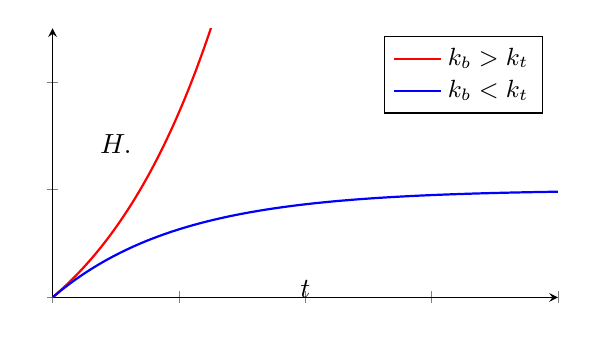
\begin{tikzpicture}
    \begin{axis}[
        width = 8cm,
        height = 5cm,
        legend pos = north east,
        x label style={at={(axis description cs:0.5,0.1)},anchor=north},
        y label style={at={(axis description cs:0.125,0.5)},rotate=270,anchor=south},
        xlabel = {$t$},
        ylabel = {$\con{H.}$},
        axis lines = left,
        ymax = 5,
        domain = 0:8,
        samples = 400,
        xticklabels={},
        yticklabels={}
    ]
    \addplot [thick, red] {2*(e^(0.5*x)-1)};
    \addlegendentry{\small{$k_b>k_t$}}
    \addplot [thick, blue] {-2*(e^(-0.5*x)-1)};
    \addlegendentry{\small{$k_b<k_t$}}
    \end{axis}
\end{tikzpicture}
\end{document}
\end{figure}
可以看到,当$k_b>k_t$时,\ce{H.}的浓度随时间指数增长,反应将在很短的时间发生,最终表现为爆炸.%
当$k_b<k_t$时,\ce{H.}的浓度随着时间增长趋于平稳,反应的速率为一常数,最终表现为稳定燃烧.
\end{document}